%; whizzy paragraph -pdf xpdf -latex ./whizzypdfptex.sh
%; whizzy-paragraph "^\\\\begin{frame}"
% latex beamer presentation.
% platex, latex-beamer でコンパイルすることを想定。 

%     Tokyo Debian Meeting resources
%     Copyright (C) 2009 Junichi Uekawa
%     Copyright (C) 2009 Nobuhiro Iwamatsu

%     This program is free software; you can redistribute it and/or modify
%     it under the terms of the GNU General Public License as published by
%     the Free Software Foundation; either version 2 of the License, or
%     (at your option) any later version.

%     This program is distributed in the hope that it will be useful,
%     but WITHOUT ANY WARRANTY; without even the implied warranty of
%     MERCHANTABILITY or FITNESS FOR A PARTICULAR PURPOSE.  See the
%     GNU General Public License for more details.

%     You should have received a copy of the GNU General Public License
%     along with this program; if not, write to the Free Software
%     Foundation, Inc., 51 Franklin St, Fifth Floor, Boston, MA  02110-1301 USA

\documentclass[cjk,dvipdfmx,12pt]{beamer}
\usetheme{Tokyo}
\usepackage{monthlypresentation}

%  preview (shell-command (concat "evince " (replace-regexp-in-string "tex$" "pdf"(buffer-file-name)) "&"))
%  presentation (shell-command (concat "xpdf -fullscreen " (replace-regexp-in-string "tex$" "pdf"(buffer-file-name)) "&"))
%  presentation (shell-command (concat "evince " (replace-regexp-in-string "tex$" "pdf"(buffer-file-name)) "&"))

%http://www.naney.org/diki/dk/hyperref.html
%日本語EUC系環境の時
\AtBeginDvi{\special{pdf:tounicode EUC-UCS2}}
%シフトJIS系環境の時
%\AtBeginDvi{\special{pdf:tounicode 90ms-RKSJ-UCS2}}

\title{Emdebian/Grip}
\subtitle{資料}
\author{岩松 信洋 iwamatu@debian.org\\IRC nick: iwamatsu}
\date{2010年4月17日}
\logo{
\includegraphics[width=8cm]{image200607/openlogo-light.eps}}

\begin{document}

\frame{\titlepage{}}

\emtext{Debian/SH4 の進捗}

\begin{frame}{Debian/SH4 の進捗}
\begin{itemize}
\item 開始: 2009年6月頃
\item まだオフィシャルサポートアーキテクチャではない。\\
squeeze + 1 でサポート予定。

\item 現時点のサポートパッケージ数: 約7700個
\item 約93\%のパッケージをビルド済み
\end{itemize}

\end{frame}

\begin{frame}
\begin{figure}[h]
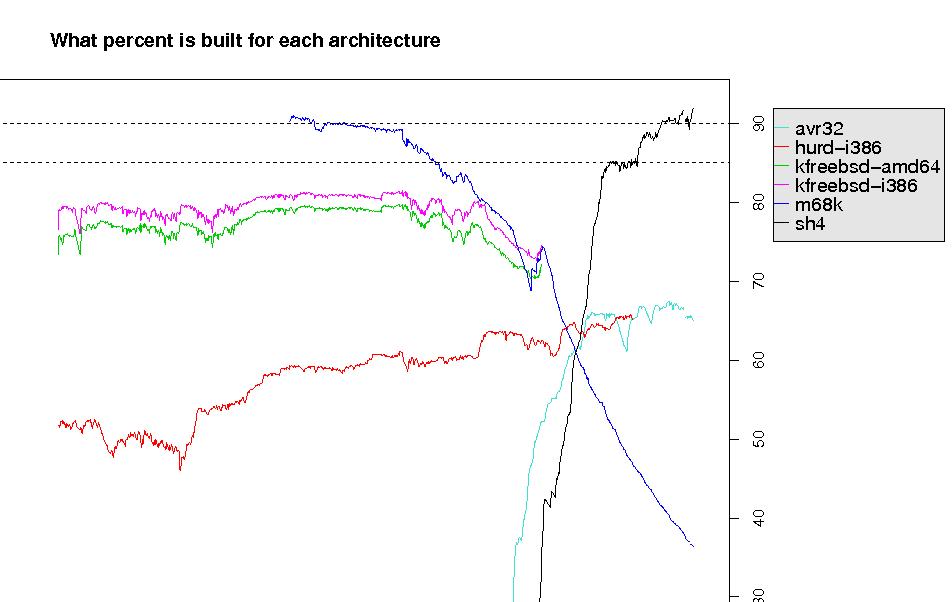
\includegraphics[height=0.7\hsize]{image201004/emdebian1.png}
\label{fig:devwork}
\end{figure}
\end{frame}

\emtext{Emdebian}

\begin{frame}{Emdebian}
\begin{itemize}
\item Pros

  \begin{enumerate}
  \item 多くのアーキテクチャをサポート、新規アーキテクチャの受け入れが容易。
  \item ライセンスに関する問題の軽減。
  \item バイナリベースディストリビューションなので、容易にソフトウェアの動作確認ができる。
  \end{enumerate}

\item Cons
  \begin{enumerate}
  \item 普通に使うとroot filesystemのサイズが大きくなるので組込みには使いづらい。
  \end{enumerate}

組込み向けサポートプロジェクト / Emdebian
\end{itemize}

\end{frame}

\begin{frame}{Emdebian}
\begin{itemize}
\item Debian パッケージのクロスコンパイル対応
\item クロスコンパイラの提供およびメンテナンス
\item 基本的にDebian オフィシャルサポートアーキテクチャをサポート
\end{itemize}
\end{frame}

\begin{frame}{Emdebianのプロジェクト}
\begin{itemize}
\item Emdebian Crush\\
Busyboxベースのroot filesystemをDebian ソースパッケージからクロスコンパ
 イルで構築するプロジェクト。しかし、今はarmelのみサポート。
\item Emdebian Grip\\
既存のパッケージを組込み向けにコンバート(必要ない情報を削る)する環境およびコンバート後のパッ
 ケージを提供する。
\end{itemize}
\end{frame}

\emtext{Emdebian / Grip}

\begin{frame}{Emdebian Grip}
必要ない情報を削るとき、手動でやってません?\\
(野良ビルドの時も)

\end{frame}

\begin{frame}[containsverbatim]{Emdebian Grip}
\begin{itemize}

\item 既存のパッケージから組込向けにパッケージをコンバートする。
\begin{commandline}
$ em_autogrip -b /target/repository/path -s apt
\end{commandline}

\item コンバート前とコンバート後のパッケージは互換性がある。
\item Grip でコンバートされたパッケージとされていないパッケージを混ぜることが
 できる。
\item Renesas SH4 も先日対応。
\item パッケージバージョンにemXが付く
\begin{commandline}
$ apt_0.7.25.3em1_sh4.deb
\end{commandline}
\end{itemize}

\end{frame}


\begin{frame}[containsverbatim]{Emdebian Grip}
\begin{itemize}

\item 例: aptパッケージをコンバートする\\

コンバート前: 1.8M apt\_0.7.25.3\_sh4.deb\\
コンバート後: 638K apt\_0.7.25.3em1\_sh4.deb

\item 何が減ったのか\\
man、ドキュメント、メッセージカタログ\\
コンバート前: 136 directories, 212 files\\
コンバート後: 37 directories, 34 files\\
\end{itemize}
\end{frame}


\begin{frame}[containsverbatim]{Emdebian Grip}

例: システム全体を Grip に置き換える\\
  対象 : パッケージ数164個の debian ベースシステム
\begin{enumerate}
\item \texttt{/etc/apt/sources} を gripに変更\\
変更前: \texttt{deb http://ftp.debian-ports.org/debian/ unstable main}\\
変更後: \texttt{deb http://www.emdebian.org/grip/ unstable main}\\
\item \texttt{apt-get update}
\item \texttt{apt-get upgrade}\\
     置き換え前: 186M \\
     置き換え後: 79M (半分に縮小)\\
\end{enumerate}
\end{frame}

\begin{frame}
\begin{minipage}[t]{0.25\hsize}
コンバート前:\\
5  bin\\
1  boot\\
1  dev\\
2  etc\\
1  home\\
9  lib\\
1  media\\
1  mnt\\
1  opt\\
\end{minipage}
\begin{minipage}[t]{0.2\hsize}
 \\
1  proc\\
1  root\\
4  sbin\\
1  selinux\\
1  srv\\
1  sys\\
1  tmp\\
108 usr\\
58 var\\
\end{minipage}
\begin{minipage}[t]{0.25\hsize}
コンバート後:\\
5  bin\\
1  boot\\
1  dev\\
2  etc\\
1  home\\
9  lib\\
1  media\\
1  mnt\\
1  opt\\
\end{minipage}
\begin{minipage}[t]{0.2\hsize}
 \\
1  proc\\
1  root\\
4  sbin\\
1  selinux\\
1  srv\\
1  sys\\
1  tmp\\
50 usr\\
11 var\\
\end{minipage}
\footnote{単位はMB}
\end{frame}



\begin{frame}[containsverbatim]{i18n の対応}
\begin{itemize}
\item Tdeb (translation) を使って提供
\item 必要なパッケージの必要な言語を選択してインストールできる 
\end{itemize}
\end{frame}


\begin{frame}[containsverbatim]{さらに削る}
\begin{itemize}
\item 必要ないプログラムを消していく\\
  Not deb package.

\item ソフトウェア機能を削る → 要再ビルド
\item Emdebian Crush を利用\\
 uClibc を使ったシステムを利用(現在開発中) 
\end{itemize}
\end{frame}

\begin{frame}[containsverbatim]{まとめ}
\begin{itemize}
\item debianでいらない情報をけずるときは、emdebian/grip で提供されている
      パッケージを使うか、em\_autogripを使う。
\item emdebian/grip は debianパッケージと互換性がある。
\item さらに削りたいときは emdebian crush を使う。
\item さらにさらに削りたいときは Openembeddedやbuildrootを使いましょう。
\item debian/sh4 のテスター募集中 
\end{itemize}


\end{frame}


\end{document}

;;; Local Variables: ***
;;; outline-regexp: "\\([ 	]*\\\\\\(documentstyle\\|documentclass\\|emtext\\|section\\|begin{frame}\\)\\*?[ 	]*[[{]\\|[]+\\)" ***
;;; End: ***
